\documentclass{article}

\usepackage[a4paper,margin=1in]{geometry}

\usepackage{mystyle}
\usepackage[sort,comma,numbers]{natbib}
\usepackage{algorithm}
\usepackage[noend]{algpseudocode}
\usepackage{hyperref}
\usepackage{todonotes}
\usepackage{algorithm}

\usepackage{tikz}
\usetikzlibrary{bayesnet}

\usepackage{subcaption}

\title{Random Fourier Features for Scaling Markov Random Fields}

\begin{document}
\maketitle

The exponential kernel, $\exp(\bx^T\by)$ with $\bx,\by\in\R^n$,
is widely used to parameterize discrete distributions.
It can be well-approximated by Random Fourier Features
(RFF):
\begin{equation}
\exp(\bx^T\by)\approx \phi(\bx)^T\phi(\by),
\end{equation}
with random projections $\phi:\R^n\to\R^d$ \citep{rawat2019linearizedsoftmax}.
Importantly, this approximation is linear, and therefore admits
reordering tricks based on the distributive and associative property
to improve the efficiency of certain operations by polynomial factors.

\section{Attention}
One such operation is attention, a popular operation used in neural networks.
Naively, attention requires quadratic time complexity.
However, the sampled softmax with RFF \citep{rawat2019linearizedsoftmax}
can be applied to compute attention with linear time complexity
\citep{choromanski2020rethinking}
(and many others, such as Random Feature Attention, LinFormers, etc.).

\subsection{Linear attention with RFF}
Given queries $\bq_j\in\R^n$, keys $\bk_i\in\R^n$, and values $\bv_i\in\R^n$ with $t\in[T],i\in[I]$,
attention computes outputs
\begin{equation}
o_t = \sum_i \frac{\exp(\bq_t^T\bk_i)\bv_i^T}{\sum_j \exp(\bq_t^T\bk_j)}.
\end{equation}
This requires $O(TIn)$ time to compute for all $o_t$.
Applying the RFF approximation, we have
\begin{equation}
o_t \approx \sum_i \frac{(\phi(\bq_t)^T\phi(\bk_i))\bv_i^T}{\sum_j\phi(\bq_t)^T\phi(\bk_j)}
= \frac{\phi(\bq_t)^T\sum_i\phi(\bk_i)\bv_i^T}{\phi(\bq_t)^T\sum_j\phi(\bk_j)}.
\end{equation}
The terms $\sum_i\phi(\bk_i)\bv_i^T$ and $\sum_j\phi(\bk_j)$ can be computed once for all queries,
reducing the time complexity of computing all $o_t$ to $O(Td+Id^2)$.

\paragraph{Matrix version}
Matrix form \citep{choromanski2020rethinking} is more informative, write up later.
Just breaks up $A$ matrix into linear decomposition,
then applies associative property of matmul.

\subsection{Approximation error}
todo

\section{Linear Chain MRFs}
The RFF approximations work well in unstructured distributions.
Can we get even tighter approximations when distributions have structure?
Does the approximation even work?
\todo{change all this}

\subsection{Drop-in substitution of kernel approximation}
We start with a linear-chain MRF:
$$p(x) \propto \prod_t \psi(x_{t-1},x_t) = \prod_t \exp(\bx_{t-1}^T\bx_t),$$
with the variables $x_t\in\mcX$ and embeddings $\bx_t\in\R^n$.
\begin{comment}
\begin{figure}[h]
\centering
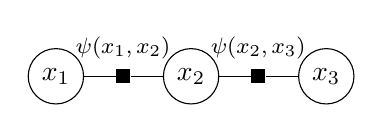
\begin{tikzpicture}
\node[latent] (x1) {$x_1$};
\node[latent, right=of x1] (x2) {$x_2$};
\node[latent, right=of x2] (x3) {$x_3$};
\factor[right=of x1] {f1} {$\psi(x_1,x_2)$} {} {};
\factor[right=of x2] {f2} {$\psi(x_2,x_3)$} {} {};
\factoredge {x1,x2} {f1} {};
\factoredge {x2,x3} {f2} {};
\end{tikzpicture}
\caption{
\label{fig:linear-chain}
}
\end{figure}
\end{comment}
As before, we approximate
$\psi_t(x_{t-1}, x_t) = \exp(\bx_{t-1}^T \bx_t) \approx \phi(\bx_{t-1})^T\phi(\bx_t)$,
with the random projection $\phi(\cdot): \R^n \to \R^d$ chosen appropriately.
To start, consider computing the partition function of a simple example with $T=3$:
\begin{equation}
\begin{aligned}
Z
&= \sum_{x_1}\sum_{x_2} \psi_1(x_1, x_2) \sum_{x_3} \psi_2(x_2, x_3) \\
&\approx \sum_{x_1}\sum_{x_2} \phi(\bx_1)^T\phi(\bx_2) \sum_{x_3} \phi(\bx_2)^T\phi(\bx_3)\\
&= \left(\sum_{x_1} \phi(\bx_1)^T\right) \left(\sum_{\bx_2} \phi(\bx_2)\phi(\bx_2)^T\right)
    \left(\sum_{x_3}\phi(\bx_3)\right).
\end{aligned}
\end{equation}
We can precompute the sum of outer products $\sum_{\bx_2}\phi(\bx_2)\phi(\bx^T)$ independently,
resulting in time complexity $O(Td^2 + T|\mcX|d^2)$ in serial,
and $O(Td^2 + |\mcX|d^2)$ if the sums of outer products can be computed in parallel.
We can also apply a divide-and-conquer approach to further
reduce time to $O(c_{\textrm{mm}}(\log T + \log |\mcX|))$ on a parallel machine,
where $c_{\textrm{mm}}(d)$ is the cost of a matrix multiplication which is polynomial in $d$.
Compared to the original time complexity of $O(T|\mcX|^2)$,
this is particularly beneficial if $d \ll |\mcX|$.

\paragraph{Matrix version}
Probably much clearer here too.
todo

\subsection{Approximation error}
todo

\section{Hidden Markov Models}
An HMM consists of transitions between latent states $p(z_t \mid z_{t-1})$
and emissions from latent states to observed words $p(x_t \mid z_t)$,
where these conditional distributions are locally normalized by definition.
The joint distribution is given by $p(x, z) = \prod_t p(z_t \mid z_{t-1})p(x_t \mid z_t)$
with a dummy state $z_0 = \epsilon$.
In order to compute the evidence of the observed words, the latent states must be
marginalized over: $p(x) = \sum_z p(x,z)$.
Applying the RFF approximation to sequence $x$ with $|x| = 2$, we have
a linear-chain MRF plus some scaling terms:
\begin{equation}
\begin{aligned}
p(x)
&= \sum_{z_1} p(z_1 \mid z_0)p(x_1 \mid z_1)  \sum_{z_2} p(z_2 \mid z_1)p(x_2 \mid z_2)\\
&= \sum_{z_1} \frac{\phi(\bz_0)^T\phi(\bz_1)}{\sum_{z_1'}\phi(\bz_0)^T\phi(\bz'_1)}
\frac{\phi(\bz_z)^T\phi(\bx_1)}{\sum_{x_1}\phi(\bz_1)^T\phi(\bx_1)}
\sum_{z_2} \frac{\phi(\bz_1)^T\phi(\bz_2)}{\sum_{z_2'}\phi(\bz_1)^T\phi(\bz_2')}
\frac{\phi(\bz_2)^T\phi(\bx_2)}{\sum_{x_2}\phi(\bz_2)^T\phi(\bx_2)}\\
%&= \sum_{z_1} \frac{\phi(\bz_0)^T\phi(\bz_1)}{\phi(\bz_0)^T\sum_{z_1'}\phi(\bz'_1)}
%\frac{\phi(\bz_1)^T\phi(\bx_1)}{\phi(\bz_1)^T\sum_{x_1}\phi(\bx_1)}
%\sum_{z_2} \frac{\phi(\bz_1)^T\phi(\bz_2)}{\phi(\bz_1)^T\sum_{z_2'}\phi(\bz_2')}
%\frac{\phi(\bz_2)^T\phi(\bx_2)}{\phi(\bz_2)^T\sum_{x_2}\phi(\bx_2)}\\
&= \left(\frac{\phi(\bz_0)^T}{\phi(\bz_0)^T\sum_{z_1'}\phi(\bz'_1)}\right)
\left(
\sum_{z_1} 
\frac{\left(\phi(\bz_1)^T\phi(\bx_1)\right)\phi(\bz_1)\phi(\bz_1)^T}
{
    \left(\phi(\bz_1)^T\sum_{x_1}\phi(\bx_1)\right)
    \left(\phi(\bz_1)^T\sum_{z_2'}\phi(\bz_2')\right)
}
\right)
\left(
\sum_{z_2} 
\frac{\left(\phi(\bz_2)^T\phi(\bx_2)\right)\phi(\bz_2)}{\phi(\bz_2)^T\sum_{x_2}\phi(\bx_2)}
\right).
\end{aligned}
\end{equation}


\section{Tree MRFs}
We proceed from first order linear-chain MRFs, where nodes only have 2 neighbours,
to the next simplest model: trees.
With tree MRFs, nodes may have more than 2 neighbours depending on the arity of the tree,
but the dependencies are still simple and exact inference is tractable.

In linear-chain MRFs all elimination orders are equivalent, as the elimination 
of a variable cannot result in the addition of any fill-in edges.
Indeed, this is the reason why divide-and-conquer strategies are possible
in the first place.
As this is not the case for tree MRFs (consider removing a node in the middle of a tree),
we cannot get the same speedups as in the linear-chain MRF.
However, speedups due to parallelization and projection are still be possible.

\subsection{RFF allows reording of tensor contraction}
Consider a star MRF with the following joint distribution:
\begin{equation}
p(x) \propto \psi(x_1, x_2) \psi(x_2, x_3) \psi(x_2, x_4),
\end{equation}
shown in Figure~\ref{fig:star-mrf}.
\begin{figure}[htb!]
\centering
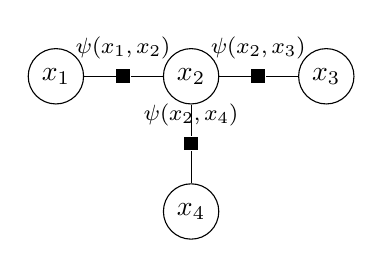
\begin{tikzpicture}
\node[latent] (x1) {$x_1$};
\node[latent, right=of x1] (x2) {$x_2$};
\node[latent, right=of x2] (x3) {$x_3$};
\node[latent, below=of x2] (x4) {$x_4$};
\factor[right=of x1] {f1} {$\psi(x_1,x_2)$} {} {};
\factor[right=of x2] {f2} {$\psi(x_2,x_3)$} {} {};
\factor[below=of x2] {f3} {$\psi(x_2,x_4)$} {} {};
\factoredge {x1,x2} {f1} {};
\factoredge {x2,x3} {f2} {};
\factoredge {x2,x4} {f3} {};
\end{tikzpicture}
\caption{
\label{fig:star-mrf}
}
\end{figure}
Elimination takes time $O(V|\mcX|^2)$, where $V$ is the number of nodes.
The time complexity can be lowered on a parallel device to $O(|\mcX|^2)$
using tensor variable elimination \citep{obermeyer2019tve}.

Applying the RFF approximation, elimination is then given by
\begin{equation}
\label{eqn:star}
\begin{aligned}
Z &= \sum_\bz \psi(x_1, x_2) \psi(x_2, x_3) \psi(x_2, x_4) \\
&\approx \sum_{x_1} \sum_{x_2} \phi(x_1)^T\phi(x_2)
    \sum_{x_3} \phi(x_2)^T\phi(x_3) \sum_{x_4} \phi(x_2)^T\phi(x_4)\\
&= \sum_{x_1} \phi(x_1)^T \sum_{x_2} \phi(x_2)
    \left(\phi(x_2)^T \sum_{x_3} \phi(x_3)\right)
    \left(\phi(x_2)^T\sum_{x_4} \phi(x_4)\right).
\end{aligned}
\end{equation}
We can pull $\phi(x_2)^T$ from the last two terms with a tensor product:
\todo{definitely something slightly weaker than the commutative property is being used here,
which is clear in the einsum version.
not sure what to call this?
is this a generalized cyclical trace property or just the tensor analogue of polynomials}
\begin{equation}
Z \approx \left(\sum_{x_1} \phi(x_1)^T \right)
\left(\sum_{x_2} \phi(x_2) \otimes\phi(x_2) \otimes \phi(x_2)  \right)
\left(\sum_{x_3} \phi(x_3)\right) 
\left(\sum_{x_4} \phi(x_4)\right),
\end{equation}
where this approximation can be computed in time $O(|\mcX|d^3)$.

Generalizing to $n$-arity trees, we can go from the original runtime of $O(E|\mcX|^2)$
for variable elimination to $O(Ed^2 + |\mcX|d^n)$ by applying the
RFF approximation and reordering contraction, where $E$ is the number of edges.

\subsection{Approximation error}

\paragraph{Tensor version, einsum version}
\todo{asdf}

\section{Application to globally normalized HMMs}
The tree example of RFF-MRFs above extends directly to globally normalized HMMs.
Consider an HMM with discrete observations $x_t \in \mcX$
and discrete latent states $z_t\in\mcZ$.
The joint distribution is given by
\begin{equation}
p(x,z) \propto \prod_t \psi(x_{t-1}, x_t) \psi(z_t, x_t)
= \prod_t \exp(\bx_{t-1}, \bx_t) \exp(\bz_t, \bx_t),
\end{equation}
with $\bx_t,\bz_t\in\R^d$.
The graphical model is given in Figure \ref{fig:hmm}.
\begin{figure}[htb!]
\centering
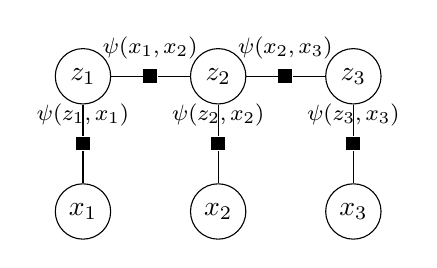
\begin{tikzpicture}
\node[latent] (z1) {$z_1$};
\node[latent, right=of z1] (z2) {$z_2$};
\node[latent, right=of z2] (z3) {$z_3$};
\node[latent, below=of z1] (x1) {$x_1$};
\node[latent, below=of z2] (x2) {$x_2$};
\node[latent, below=of z3] (x3) {$x_3$};
\factor[right=of z1] {f12} {$\psi(x_1,x_2)$} {} {};
\factor[right=of z2] {f23} {$\psi(x_2,x_3)$} {} {};
\factor[below=of z1] {g1} {$\psi(z_1,x_1)$} {} {};
\factor[below=of z2] {g2} {$\psi(z_2,x_2)$} {} {};
\factor[below=of z3] {g3} {$\psi(z_3,x_3)$} {} {};
\factoredge {z1,z2} {f12} {};
\factoredge {z2,z3} {f23} {};
\factoredge {x1,z1} {g1} {};
\factoredge {x2,z2} {g2} {};
\factoredge {x3,z3} {g3} {};
\end{tikzpicture}
\caption{
\label{fig:hmm}
}
\end{figure}

To compute the partition function we perform the same computation
as in Equation~\ref{eqn:star}:
\begin{equation}
\begin{aligned}
Z &= \sum_x\sum_z \prod_t \psi(x_{t-1}, x_t)\psi(z_t, x_t)\\
&\approx
\left(\left(\sum_{x_1} \phi(\bx_1)^T \right) \left(\sum_{z_1} \phi(\bz_1)\otimes \phi(\bz_1) \right)\right)\\
&\qquad \cdot \left(\left(\sum_{x_2} \phi(\bx_2) \right) \left(\sum_{z_2} \phi(\bz_2)\otimes \phi(\bz_2)\otimes\phi(\bz_2) \right)\right)\\
&\qquad \cdot \left(\left(\sum_{x_3} \phi(\bx_3) \right) \left(\sum_{z_3} \phi(\bz_3)\otimes \phi(\bz_3)\otimes\phi(\bz_3) \right)\right)
\cdots\\
&\qquad \cdot \left(\left(\sum_{z_T} \phi(\bz_T)\otimes \phi(\bz_T) \right)\left(\sum_{x_T} \phi(\bx_T) \right) \right).
\end{aligned}
\end{equation}
\todo{probably take out $x_3$}
Again, each of the summations and summands can be computed in parallel.
\todo{expand / finish}

\section{HSMM}

\section{Application to WCFGs}
\begin{algorithm}[H]
  \begin{algorithmic}[1]
    \Function{INSIDE}{$\pi$, $w$}
      \State initialize all $\beta[\cdot_\cdot^\cdot]$ to 0
      \For{$k := 1 \to n$} \Comment{width-1 constituents}
        \For{$A\in \mathcal{N}$}
        \State{$\beta[A_{k-1}^k]+= \pi (A\to w_k)$} \Comment{$O(K^2)$}  
        \EndFor    
    \EndFor
    \For{$\text{width} := 2 \to n$} \Comment{wider constituents}
      \For{$i := 0 \to n-\text{width}$} \Comment{start point}
        \State $k := i + \text{width}$ \Comment{end point}
        \For{$j := i + 1 \to k-1$} \Comment{midpoint}
          \For{$A,B,C \in \mathcal{N}$}
            \State $\beta [A_{i}^k]+ = \pi (A \to B C) \beta[B_i^j] \beta[C_j^k]$
          \EndFor
        \EndFor
      \EndFor
    \EndFor
    \State\Return $Z:=\beta[\text{ROOT}_0^n]$ 
    \EndFunction
  \end{algorithmic}
  \caption{\label{algo:inside}The inside algorithm from \cite{eisner2016inside}}
\end{algorithm}
The inside algorithm is outlined in Algorithm~\ref{algo:inside}. With $n$ words and $|\mathcal{N}|$ non-terminals, the complexity is
\begin{equation}
    O(n^3 |\mathcal{N}|^3),
\end{equation}
where the major complexity comes from the updates at line 11: $\beta [A_{i}^k]+ = \pi (A \to B C) \beta[B_i^j] \beta[C_j^k]$.

%To reduce the computation complexity, we need to leverage shared computations arises from the parameterization of rule probabilities $\pi (A \to B C)$. 

If we make the assumption that
\begin{equation}
    \pi (A \to B C) = \frac{\phi(A, B) \cdot \mathbf{\psi}(A, C)}{\sum_{B'C'} \phi(A, B') \cdot \psi(A, C')},
\end{equation}
where $\phi$ and $\psi$ are feature functions that maps $A, B$ and $A, C$ to vectors of length $r$, then we can calculate line 11 as

\begin{align}
    \beta [A_{i}^k] & = \sum_{BC}\frac{\phi(A, B) \cdot \mathbf{\psi}(A, C) \beta[B_i^j] \beta[C_j^k]}{\sum_{B'C'} \phi(A, B') \cdot \psi(A, C')} \\
    &= \frac{(\sum_B \beta[B_i^j] \phi(A, B)) \cdot (\sum_C \mathbf{\psi}(A, C)  \beta[C_j^k])}{(\sum_{B'} \phi(A, B') )\cdot (\sum_{C'}\psi(A, C'))} ,
\end{align}
and reduce the total complexity to 
\begin{equation}
     O(n^3 |\mathcal{N}|^2 r).
\end{equation}

Note that the parameterization here is different from \cite{kim2019compound}, where $\pi (A \to B C)$ is parameterized as

\begin{equation}
    \pi (A \to B C) = \frac{\exp(\mathbf{u}_{BC} \mathbf{w}_A + \mathbf{b}_{BC})}{\sum_{B'C'} \exp(\mathbf{u}_{B'C'} \mathbf{w}_A + \mathbf{b}_{B'C'})},
\end{equation}
where $\mathbf{u}_{BC}$ is the embedding vector of $(B, C)$, and $\mathbf{w}_A$ is the embedding vector of $A$.

\section{Application to MRF-LM}
n-gram potentials (yacine's paper?)
loop over different lengths to compute partition fn?

\section{Numerical Stability}
todo

\bibliographystyle{plainnat}
\bibliography{bib}

\end{document}
